\marginnote{E-Exp-3}

This experiment mirrors Experiment 2, but focussing on instructions that did not use a number. We manipulated vagueness and the selection task (comparison and matching). In order to implement the experiment without mentioning numbers in the instructions, we changed the sequence of each trial to include a `target' (i.e., a dot array of a particular cardinality) before the array, so that we could then refer to the target's cardinality in the instruction using expressions like \emph{the same number of dots as the target}; \emph{fewer dots than the target}. An example of this sequence is given in Figure \ref{Experiment3examplestimulus}. This presentation of a target before the main body of the trial shares some features with \citeauthor[Experiment 2]{Izard20081221}, although in that experiment participants were told the cardinality of the target (called an \emph{inducer} in that paper) whereas in our experiment we did not tell participants the cardinality of the prime array. An item was thus a combination of a target dot array, an instruction that did not contain a number, and a set of dot arrays taking their cardinalities from the same triples used in Experiments 1 and 2. Table \ref{instructionsE-exp-3} spells out how the instructions were constrained not to mention a numeral and gives examples of targets.

\begin{figure}[htbp]
\centering
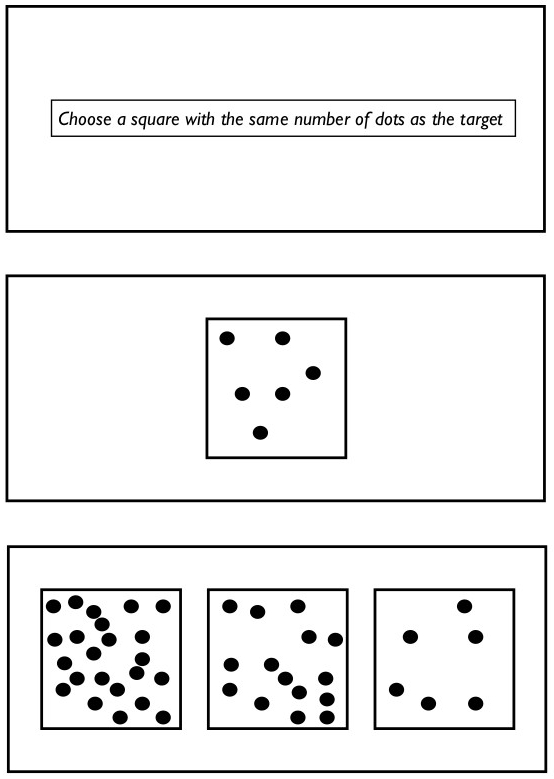
\includegraphics[width=.5\textwidth]{figures/Ee3-flow.jpg}
\caption{Experiment 3 example stimulus}
\label{Experiment3examplestimulus}
\end{figure}

\begin{table}
\centering
\caption{Experiment 3 instructions arranged by condition. The instructions given in the table started with ``Choose a square with \ldots"}
\label{instructionsE-exp-3}
\resizebox{\textwidth}{!}{\begin{tabular}{ccccll}
\hline\noalign{\smallskip}
Item & Target & Quantity & Selection & Crisp & Vague \\ 
\noalign{\smallskip}\hline\noalign{\smallskip}
06:15:24 &   6 & Small & Matching 	& the same number of dots as the target & NA \\ 
06:15:24 &  10 & Small & Matching 	& NA & about the same number of dots as the target \\ 
06:15:24 &  10 & Large & Comparison & more dots than the target & far more dots than the target \\ 
06:15:24 &  20 & Small & Comparison & fewer dots than the target & far fewer dots than the target \\ 
06:15:24 &  20 & Large & Matching 	& NA & about the same number of dots as the target \\ 
06:15:24 &  24 & Large & Matching 	& the same number of dots as the target & NA \\ 
\noalign{\smallskip}\hline\noalign{\smallskip}
16:25:34 &  16 & Small & Matching 	& the same number of dots as the target & NA \\ 
16:25:34 &  20 & Small & Matching 	& NA & about the same number of dots as the target \\ 
16:25:34 &  20 & Large & Comparison & more dots than the target & far more dots than the target \\ 
16:25:34 &  30 & Small & Comparison & fewer dots than the target & far fewer dots than the target \\ 
16:25:34 &  30 & Large & Matching 	& NA & about the same number of dots as the target \\ 
16:25:34 &  34 & Large & Matching 	& the same number of dots as the target & NA \\ 
\noalign{\smallskip}\hline\noalign{\smallskip}
26:35:44 &  26 & Small & Matching 	& the same number of dots as the target & NA \\ 
26:35:44 &  30 & Small & Matching 	& NA & about the same number of dots as the target \\ 
26:35:44 &  30 & Large & Comparison & more dots than the target & far more dots than the target \\ 
26:35:44 &  40 & Small & Comparison & fewer dots than the target & far fewer dots than the target \\ 
26:35:44 &  40 & Large & Matching 	& NA & about the same number of dots as the target \\ 
26:35:44 &  44 & Large & Matching 	& the same number of dots as the target & NA \\ 
\noalign{\smallskip}\hline\noalign{\smallskip}
36:45:54 &  36 & Small & Matching 	& the same number of dots as the target & NA \\ 
36:45:54 &  40 & Small & Matching 	& NA & about the same number of dots as the target \\ 
36:45:54 &  40 & Large & Comparison & more dots than the target & far more dots than the target \\ 
36:45:54 &  50 & Small & Comparison & fewer dots than the target & far fewer dots than the target \\ 
36:45:54 &  50 & Large & Matching 	& NA & about the same number of dots as the target \\ 
36:45:54 &  54 & Large & Matching 	& the same number of dots as the target & NA \\ 
\noalign{\smallskip}\hline
\end{tabular}}
\end{table}

\subsection{Hypotheses (Experiment 3)}

For Experiment 3, we hypothesised:

\begin{description}
	\item [Hypothesis 1] Vague instructions are easier for the reader than crisp ones (main effect of vagueness)
	\item [Hypothesis 2] Comparison is easier for the reader than matching (main effect of selection)
	\item [Hypothesis 3] Effects of vagueness differ depending on whether selection is matching or comparison (interaction effect selection x vagueness, and focussed comparisons at each level of selection).
\end{description}

\subsection{Results (Experiment 3)}
40 volunteers participated. The results showed that vagueness was beneficial for comparison but detrimental for matching (the same as Experiment 2) even when no numbers were allowed in the instructions. Figure \ref{resultsE-exp-3} shows the means by condition. Our findings were as follows:

\begin{figure}[htbp]
\centering
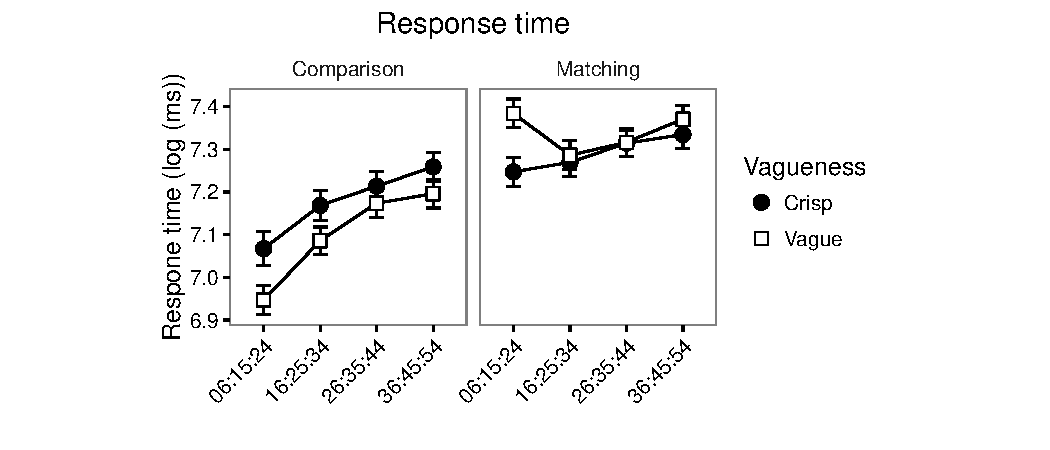
\includegraphics[width=\textwidth]{figures/Ee3-rtplot-1.pdf}
\caption{Mean response times by condition for Experiment 3 where all instructions were verbal}
\label{resultsE-exp-3}
\end{figure}

\begin{description}
	\item [Test of hypothesis 1] Vague instructions resulted in faster responses than crisp instructions on average. However this difference was not significant in the full model ($\beta=-0.015$, $se=0.0097$, $t=-1.58$, $p=0.119$). Using Levy's method \citep{Levy:MainEffectsInteractions} to test for main effects in the presence of higher-order interactions, by doing model comparison between a null model that included all interaction terms involving Vagueness but leaving out a term for the main effect of Vagueness, against a full model that differed only by including Vagueness as a main effect, showed that the full model was no better than the reduced model (df=1, p=0.118) - consituting more evidence that Vagueness did not exert a significant main effect on response times. 
	\item [Test of hypothesis 2] comparison instructions resulted in faster responses than matching instructions, and the difference was significant ($\beta=0.176$, $se=0.0168$, $t=10.51$, $p<0.001$).
	\item [Test of hypothesis 3] Although Vagueness did not exert a significant main effect, Vagueness did exert effects in interactions with some other variables: the interaction between Vagueness and Selection task  was significant ($\beta=0.123$, $se=0.0166$, $t=7.42$, $p<0.001$), suggesting that Vagueness speeded RTs in the comparison condition but slowed them down in the matching task. 
	Separate analyses at each level of selection \ldots
	%provided evidence that vague instructions resulted in faster responses than crisp instructions for the comparison condition (p<0.01); and slower responses than crisp instructions in the matching condition (p<0.01). 
	%
%Separate analyses of the effect of vagueness were conducted for the comparison task and for the matching task using Bonferroni-adjusted significance thresholds. 
%In the comparison task, vagueness resulted in faster response times ($\beta=-0.08$, $se=0.02$, $t=-4.3$, $p<0.0001$). 
%In the matching task vagueness slowed response times ($\beta=0.05$, $se=0.01$, $t=3.7$, $p=0.0004$). 
%These results are in the same direction as Experiment 2.
\end{description}

\subsection{Discussion (Experiment 3)}
Once again, the cost reduction account was wrong to predict main effect advantages for vagueness, and wrong to predict that vagueness should be beneficial at each level of the selection task: however vagueness was advantageous in the comparison task.


